\documentclass[12pt,letterpaper]{article}
\usepackage{preamble}
\usepackage{siunitx}
\usepackage{adjustbox}
\usepackage{enumitem}
%%%%%%%%%%%%%%%%%%%%%%%%%%%%%%%%%%%%%%%%%%
%%%% Edit These for yourself
%%%%%%%%%%%%%%%%%%%%%%%%%%%%%%%%%%%%%%%%%%

\newcommand{\mathsym}[1]{{}}
\newcommand{\unicode}[1]{{}}

\newcommand\course{Graduate Modelling 2 MAT 5460}
\newcommand\hwnumber{2}
\newcommand\userID{Aaron Kim}
\def\changemargin#1#2{\list{}{\rightmargin#2\leftmargin#1}\item[]}
\let\endchangemargin=\endlist 

\theoremstyle{definition}
\newtheorem*{thm}{Theorem}

\renewcommand\thesection{\arabic{section}}
\renewcommand\thesubsection{\thesection.\arabic{subsection}}



\begin{document}
\section*{Problem 11}
For the following systems determine if the equilibrium point $x^*=0$ is semi-asymptotically stable from the left or the right.
\begin{enumerate}[label=(\roman*)]
    \item $\displaystyle x(n+1) = \big(x(n)\big)^3 + \big(x(n)\big)^2 + x(n)$
    \item $\displaystyle x(n+1) = \big(x(n)\big)^3 - \big(x(n)\big)^2 +x(n)$
\end{enumerate}

\textbf{Attempt:}
\begin{changemargin}{.5cm}{0cm}

\begin{enumerate}[label=(\roman*)]
    \item 
    To check the semi-asymptotic stability, we need to know three things:
    \begin{itemize}
        \item what are the equilibrium points, $x^*$.
        \item Do the equilibrium points satisfy the definition of semi-stable: 
        An equilibrium point $x^*$ of $x(n+1) = f(x(n))$ is semistable from the right if given $\varepsilon>0$ there exists a $\delta>0$ such that if $x(0)>x^*$, $x(0)-x^*<\delta$, then $x(n)-x^*<\varepsilon$. 
        
        \item If the equilibrium points are semi-stable, do they satisfy the definition of semi-asymptotic stability:
        
        If $\displaystyle \lim_{n\rightarrow \infty} x(n) = x^*$, whenever $x(0)-x^*<\eta \; \{(x^* - x(0))<n\}$, then $x^*$ is said to be semi-asymptotically stable from the right. If $f'(x^*)=1$ and 
        \begin{itemize}
            \item $f''(x^*) <0$, then $x^*$ is semiasympotically stable from the right.
            \item $f''(x^*) >0$, then $x^*$ is semiasympotically stable from the left.
        \end{itemize}
    \end{itemize}
    Since I am lazy, and I can't figure out how to do the \textit{actual} analysis (I tried, but couldn't get the definitions to work), we are just going to use the last 2 conditions.

    \begin{equation*}
        f'(0) = 3(0^2) + 2(0) +1 = 1
    \end{equation*}
    \begin{equation*}
        f''(0) = 6(0) + 2 = 2
    \end{equation*}
    So this is semi-asymptotically stable from the left.
    

  \item  Similarly,
      \begin{equation*}
        f'(0) = 3(0^2) - 2(0) +1 = 1
    \end{equation*}
    \begin{equation*}
        f''(0) = 6(0) - 2 = -2
    \end{equation*}
    So this is asymptotically stable from the right.

\end{enumerate}

\end{changemargin}

\newpage

\section*{Problem 12}
Consider the logistic equation:

\begin{equation*}
    x(n+1) = \mu x(n) (1-x(n))
\end{equation*}

\begin{enumerate}[label=(\roman*)]
    \item Let $\mu = 3.4$ and $x(0) = 0.45$. Show that we get a $2$-periodic point (compute the periodic orbit).
    \item Let $\mu=3.5$ and $x(0) =0.5$. Show that we get a 4-periodic point. (compute the periodic orbit). Provide the code you used.
\end{enumerate}

\textbf{Attempt:}
\begin{changemargin}{.5cm}{0cm}

\begin{enumerate}
    \item we get the values, $0.451965325993535,   0.842155078316515$
    \lstinputlisting[caption={2 values}]{matlab_files/problem_12a.m}
    \item we get the values:
    \begin{equation*}
        0.500884210307218 ,  0.874997263602464  , 0.382819683017324  , 0.826940706591439
    \end{equation*}
    \lstinputlisting[caption={2 values}]{matlab_files/problem_12b.m}
\end{enumerate}

\end{changemargin}
\newpage


\section*{Problem 13}

Consider the tent map:

\begin{align*}
    \text{Let} \quad f(x) = \begin{cases} 
    2x, & \text{ for } 0\leq x \leq\frac{1}{2}\\
    2(1-x), & \text{ for } \frac{1}{2}<x\leq 1.
    \end{cases}
\end{align*}
The tent map iteration is given by:
\begin{equation*}
    x(n+1) = f(x(n))
\end{equation*}
Let $y(n+1) = g (y(n))$, with $g(y) = f^2(y)=f(f(y))$
\begin{enumerate}[label=(\alph*)]
    \item Obtain an explicit form for the function $g(x)$.
    \item Find the fixed points of $g$.
    \item Determine the two-cycles of $f$.
\end{enumerate}



\textbf{Attempt:}

    \begin{changemargin}{.5cm}{0cm}
        \begin{enumerate}[label=(\alph*)]
    \item
    we know that $g(x) = f(f(x))$, so we must put $2x$ into each, and $2(1-x)$ into each, and adjust the initial intervals. This gives us: \begin{equation*}
        g(x) = \begin{cases}
         2(2(x)), & 0\leq x < \frac 1 4\\
         2(1-(2x)) & \frac 1 4 \leq x < \frac 1 2 \\
         2(1-2(1-x))) & \frac 1 2 \leq x < \frac 3 4\\
         2(2(1-x)) & \frac 3 4 \leq x \leq 1
        \end{cases}
    \end{equation*}
    
    
    \item Our fixed points are:
    \begin{align*}
         \begin{cases}
         4x^*-x^*=0, & 0\leq x < \frac 1 4\\
         2-4x^* - x^* = 0 & \frac 1 4 \leq x < \frac 1 2 \\
         4x^*-2 - x^*=0 & \frac 1 2 \leq x < \frac 3 4\\
         4-4x^* -x^*=0 & \frac 3 4 \leq x \leq 1
        \end{cases}
    \end{align*}
    \begin{align*}
         \begin{cases}
         x^*=0, & 0\leq x < \frac 1 4\\
         x^*=\frac 2 5 & \frac 1 4 \leq x < \frac 1 2 \\
         x^*=\frac 2 3  & \frac 1 2 \leq x < \frac 3 4\\
         x^* = \frac 4 5  & \frac 3 4 \leq x \leq 1
        \end{cases}
    \end{align*}
    \item The two cycles are $.8,.4$.
    \lstinputlisting[caption={2 values}]{matlab_files/problem_13c.m}
\end{enumerate}

    \end{changemargin}


%\begin{figure}[H]
%    \centering
%    \includegraphics[width=.7\textwidth]{images/Problem_1_extrea.png}
%    \caption{Plot toward the limit where $100 to 6285$ skipping every 100 values}
%    \label{fig:fig2}
%\end{figure}


\newpage

%

\section*{Problem 14}
Recall that the tent map problem:
\begin{equation*}
    x(n+1) = f\big(x(n)\big), \text{ with } f(x)\begin{cases}
    2x, & \text{ if } 0\leq x \leq \frac 1 2\\
    2(1-x),  &\text{ if } \frac 1 2 < x \leq 1
    \end{cases}
\end{equation*}
What is the stability of the two cycles?

\textbf{Attempt:}

\begin{changemargin}{.5cm}{0cm}
    We can apply the following Theorem:
    
    \fbox{\begin{minipage}{\textwidth}\textbf{Theorem 1.21:} 

Let $O(b) = \{b=x(0), x(1), \dots, x(k-1)\}$ be a $k$-cycle of a continuously differentiable function $f$. Then the following statements hold:

\begin{enumerate}[label = (\roman*)]
    \item The $k$-cycle $O(b)$ is asymptotically stable if:
    \begin{equation*}
        \left|f'\big(x(0)\big)f'\big(x(1)\big)\dots f'\big(x(k-1\big) \right|<1
    \end{equation*}
    \item The $k$-cycle $O(b)$ is asymptotically unstable if:
    \begin{equation*}
        \left|f'\big(x(0)\big)f'\big(x(1)\big)\dots f'\big(x(k-1\big) \right|>1
    \end{equation*}
\end{enumerate}
\end{minipage}}
    
    Then 
    \begin{equation*}
        |f'(.4)f'(.8)| = \left|2*(-2) \right| = 4>1
    \end{equation*}
    So this is asymptotically unstable.
    
\end{changemargin}

\newpage

\section*{Problem 15}

Consider the function $B(x)$ (Baker's function) given by:

\begin{equation*}
    B(x) = \begin{cases}
    2x, & \text{ if } 0\leq x \leq \frac 1 2 \\
    2x-1, & \text{ if } \frac 1 2 < x \leq 1
    \end{cases}
\end{equation*}

Sketch the graph of $B^2$ and find the two-cycles of $B$

    
  \textbf{Attempt:}
    \begin{changemargin}{.5cm}{0cm}
    
    \begin{enumerate}[label=(\alph*)]
    \item
    we know that $g(x) = f(f(x))$, so we must put $2x$ into each, and $2x-1$ into each, and adjust the initial intervals. This gives us: \begin{equation*}
        g(x) = \begin{cases}
         2(2(x)), & 0\leq x < \frac 1 4\\
         2(2x)-1 & \frac 1 4 \leq x < \frac 1 2 \\
          2(2x-1)& \frac 1 2 \leq x < \frac 3 4\\
         2(2x-1)-1 & \frac 3 4 \leq x \leq 1
        \end{cases}
    \end{equation*}
    \begin{figure}[H]
        \centering
       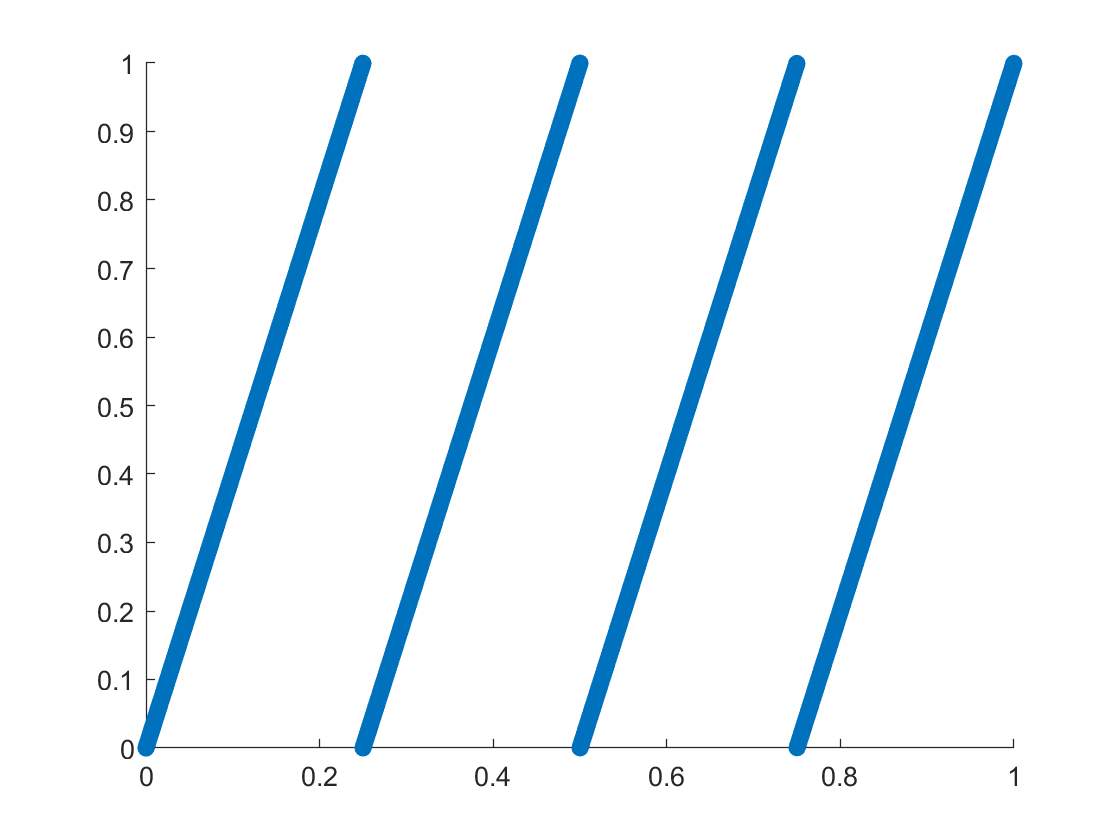
\includegraphics[width=.6\textwidth]{images/problem_15_b2.png}
        \caption{plot of $B^2$}
        \label{fig:b2}
    \end{figure}
    
    \item Our fixed points are:
    \begin{align*}
         \begin{cases}
         4x^*-x^*=0, & 0\leq x < \frac 1 4\\
         4x^* -1 - x^* = 0 & \frac 1 4 \leq x < \frac 1 2 \\
         4x^*-2 - x^*=0 & \frac 1 2 \leq x < \frac 3 4\\
        4x^* -3-x^*=0 & \frac 3 4 \leq x \leq 1
        \end{cases}
    \end{align*}
    \begin{align*}
         \begin{cases}
         x^*=0, & 0\leq x < \frac 1 4\\
         x^*=\frac 1 3 & \frac 1 4 \leq x < \frac 1 2 \\
         x^*=\frac 2 3    & \frac 1 2 \leq x < \frac 3 4\\
         x^* = 1  & \frac 3 4 \leq x \leq 1
        \end{cases}
    \end{align*}
    \item Since $x^*=0,1$ are solutions of $B(x)$, they cannot be solutions, therefore the 2-cycle is given by $\frac{1}{3},\frac{2}{3}$
    
    We can see these plotted here:
    \begin{figure}[H]
        \centering
        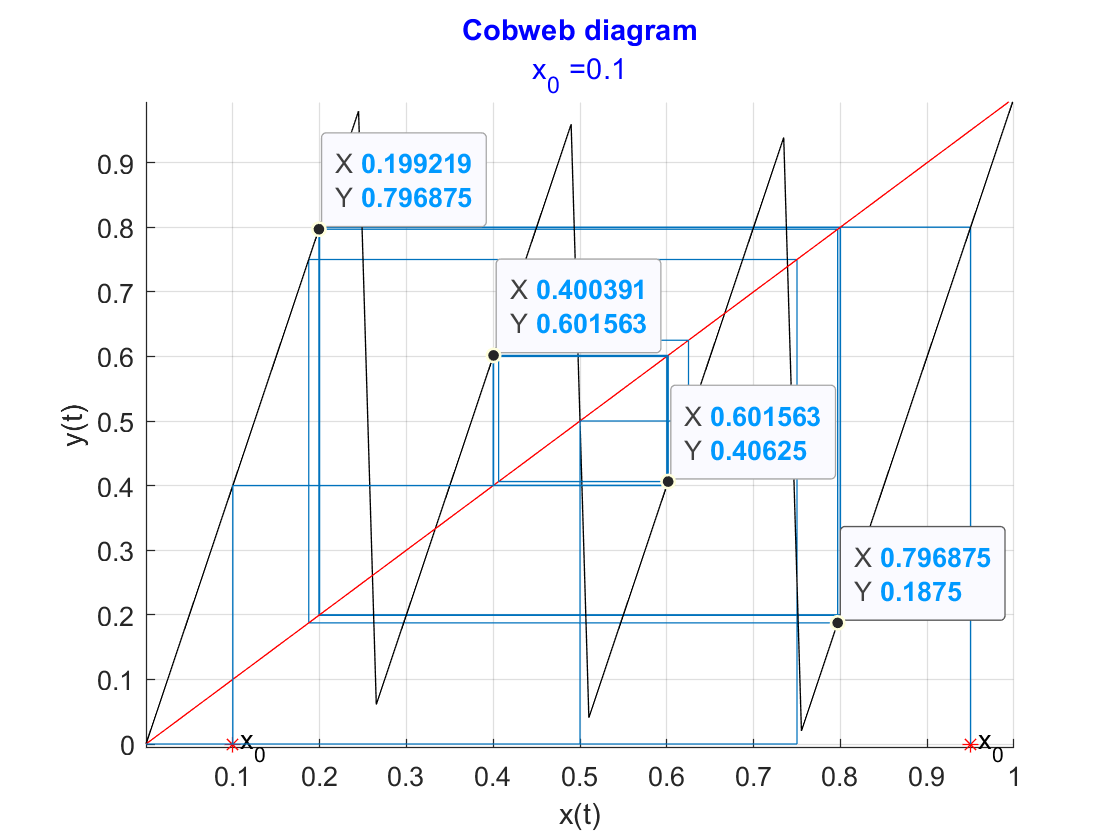
\includegraphics[width=.6\textwidth]{images/problem_15_cycles.png}
        \caption{An image of the cycles (code included at the end)}
        \label{fig:b2cycles}
    \end{figure}
\end{enumerate}


    \end{changemargin}

\section*{Problem 16}

what is the stability of the two cycle for $\mu = 1 +\sqrt{6}$? Justify your answer.

\textbf{Attempt:}
\begin{changemargin}{.5cm}{0cm}
    $F_\mu (x) = \mu x(1-x)$, and so 
    \begin{align*}
        [F^2_\mu(x(0)) ]' &= F'_\mu(x(0))F'_\mu(x(1))\\
        &=\mu(1-2x(0))\mu(1-2x(1))
        \\
       &=\mu^2(1-2x(0))(1-2x(1))
    \end{align*}
    If:
    \begin{equation*}
        x(0) = \frac{\left[ (1+\mu) -\sqrt{(\mu-3)(\mu+1)} \right]}{2\mu}
    \end{equation*}
    \begin{equation*}
        x(1) = \frac{\left[ (1+\mu) +\sqrt{(\mu-3)(\mu+1)} \right]}{2\mu}
    \end{equation*}

    We can write this as:
    \begin{equation*}
       \mu^2\left(1-2\frac{\left[ (1+\mu) -\sqrt{(\mu-3)(\mu+1)} \right]}{2\mu}\right)\left(1-2\frac{\left[ (1+\mu) +\sqrt{(\mu-3)(\mu+1)} \right]}{2\mu}\right)
    \end{equation*}
    simplifying further:
    \begin{equation*}
       \mu^2\left(\frac{\mu-\left[ (1+\mu) -\sqrt{(\mu-3)(\mu+1)} \right]}{\mu}\right)\left(\frac{\mu-\left[ (1+\mu) +\sqrt{(\mu-3)(\mu+1)} \right]}{\mu}\right)
    \end{equation*}
    \begin{equation*}
       \left(\mu-\left[ (1+\mu) -\sqrt{(\mu-3)(\mu+1)} \right]\right)\left(\mu-\left[ (1+\mu) +\sqrt{(\mu-3)(\mu+1)} \right]\right)
    \end{equation*}
    \begin{equation*}
       \left(\left[ -1 +\sqrt{(\mu-3)(\mu+1)} \right]\right)\left(\left[ -1-\sqrt{(\mu-3)(\mu+1)} \right]\right)
    \end{equation*}
    \begin{equation*}
       \left(\left[ 1 - (\mu-3)(\mu+1) \right]\right)
    \end{equation*}
    \begin{equation*}
       \left(\left[ 1- \mu^2+2\mu+3 \right]\right)
    \end{equation*}
    \begin{equation*}
       \left(\left[ 4 - (1+\sqrt{6})^2+2(1+\sqrt{6}) \right]\right)
    \end{equation*}
    \begin{equation*}
       \left(\left[ 4 - 1-2\sqrt{6}-6+2+2\sqrt{6}) = -1 \right]\right)
    \end{equation*}
    To assess the stability let's first try (\textbf{Thm 1.16}) and check the first derivative of our function:
    \begin{align*}
        F''(x) &= [F'(x(0))F'(x(1))]'\\
        &= F''(x(0))F'(x(1))+F'(x(0))F''(x(1))\\
        &= -2\mu( F'(x(1))+F'(x(0)))
    \end{align*}
    \begin{align*}
        F'''(x) &= [F'(x(0))F'(x(1))]''\\
        &= [F''(x(0))F'(x(1))+F'(x(0))F''(x(1))]'\\
        &= [-2\mu F'(x(1))-2\mu F'(x(0))]'\\
        &= 4\mu^2 +4\mu^2
    \end{align*}
    \begin{align*}
        Sf = -f'''(x^*)-\frac 3 2 (f''(x^*))^2 = -8\mu^2 - \frac{3}{2}(-2\mu(-1))^2
    \end{align*}
    \begin{equation*}
        =-8\mu^2-3\mu^2= -11(7+2\sqrt{6})<0
    \end{equation*}
    so we know that this is asymptotically stable. 
    
\end{changemargin}


\section*{Problem 17}

Iterate $x(n+1) = F_\mu \big( x(u) \big)$ for a large number of iterations. Plot the last portion of the sequence $\{x(n)\}$ as a function of $\mu$ to get a bifurcation diagram of $F_\mu$

    
\textbf{Attempt:}
\begin{changemargin}{.5cm}{0cm}
    \begin{figure}[H]
        \centering
        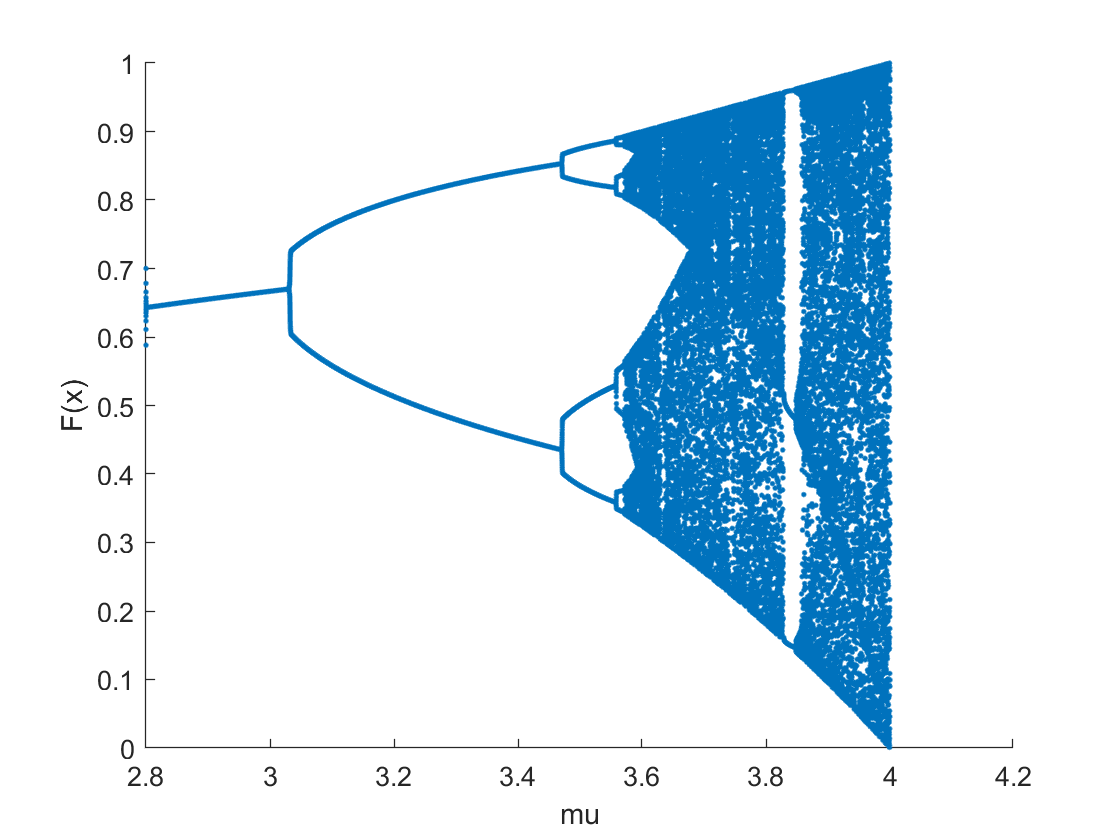
\includegraphics[width=.6\textwidth]{images/problem_17.png}
        \caption{Bifurcation diagram}
        \label{fig:bifurcation}
    \end{figure}
    \lstinputlisting[caption={bifurcation}]{matlab_files/problem_17.m}
\end{changemargin}


\section*{Problem 18}
Show that:
\begin{equation*}
    E^k x(n) = \sum_{i=0}^k {k \choose i} \Delta^{k-i}x(n)
\end{equation*}

\textbf{Attempt:}
\begin{changemargin}{.5cm}{0cm}
    From before we know that $\Delta = E-I$, so using the previous proof:
    \begin{align*}
        \Delta^kx(n)&=(E-I)^kx(n)\\
        &=\sum_{i=0}^k(-1)^i{k\choose i}E^{k-i}x(n)\\
        &=\sum_{i=0}^k(-1)^i{k\choose i}x(n+k-i)
    \end{align*}

    Since $E=\Delta + I$, and $E^k= (\Delta + I)^k$, and $\displaystyle (a+b)^n = \sum_{k=0}^n {n\choose k} a^{n-k}b^k$ :
    \begin{align*}
        E^k&=(\Delta + I)^k\\
        &=\sum_{i=0}^k{k \choose i} \Delta^{k-i}(I)^i
    \end{align*}
    Then:
    \begin{align*}
        E^kx(n) &=\sum_{i=0}^k{k \choose i} \Delta^{k-i}(I)^ix(n)\\
        E^kx(n) &=\sum_{i=0}^k{k \choose i} \Delta^{k-i}(I)x(n)\\
        E^kx(n) =\sum_{i=0}^k{k \choose i} \Delta^{k-i}x(n)\\
    \end{align*}
\end{changemargin}

\section*{Problem 19}
Show that $E$ and $\Delta$ are linear operators. That is, show that for all constants $a$ and $b$:
\begin{align*}
    \Delta[ax(n)+by(n)] &=a\Delta x(n) + b\Delta y(n)\\
    &\text{ and}\\
    E[ax(n) + by(n)]&= aEx(n) + bEy(n)
\end{align*}

\textbf{Attempt:}

\begin{changemargin}{.5cm}{0cm}
\begin{align*}
    a\Delta[x(n)]+b\Delta[y(n)] &= a[x(n+1) -x(n)] +b[y(n+1)-y(n)]\\
    &=[ax(n+1) -ax(n)] +[by(n+1)-by(n)]\\
    &=[ax(n+1)+by(n+1) ] -[ax(n)+by(n)]\\
    &=\Delta [ax(n)+by(n)]
\end{align*}
\begin{align*}
    E[ax(n) + by(n)]&= [ax(n+1) + by(n+1)]\\
    &=a[x(n+1)]+b[y(n+1)]\\
    &=a E[x(n)]+b E[y(n)]
\end{align*}
    
\end{changemargin}
    
\section*{Problem 20}
Prove that the following statements hold:

\begin{enumerate}[label = (\roman*)]
    \item $\displaystyle \sum_{i=n_0}^{n-1}\Delta x(n) = x(n) - x(n_0)$
    \item $\displaystyle \Delta \left( \sum_{k=n_0}^{n-1} x(k) \right) = x(n)$
\end{enumerate}
\textbf{Attempt:}
\begin{changemargin}{.5cm}{0cm}
    \begin{enumerate}[label = (\roman*)]
    \item \begin{align*}
       \sum_{i=n_0}^{n-1}\Delta x(n)&= \sum_{i=n_0}^{n-1}x(i+1)-x(i)\\
       &= \sum_{i=n_0}^{n-1}-x(i)+x(i+1)\\
       &=[-x(n_0)+x(n_0+1)] +[-x(n_0+1) +x(n_0+2)] + \dots\\ &+[-x(n-2)+x(n-2+1)]+ [-x(n-1)+x(n-1+1)] \\
    \end{align*}  
    But it is easy to observe that the terms between cancel:
    \begin{align*}
        &=-x(n_0)+[x(n_0+1) -x(n_0+1)] +[x(n_0+2) -x(n_0+2)] \dots\\ &[x(n-2)-x(n-2)]+[x(n-2+1)+ -x(n-1)]+x(n-1+1) \\
        &= -x(n_0)+x(n)
    \end{align*}
    So we get:$\displaystyle \sum_{i=n_0}^{n-1}\Delta x(n) = x(n) - x(n_0)$
    
    \item 
    
    \begin{align*}
        \Delta \left( \sum_{k=n_0}^{n-1} x(k) \right)&=\\
        &= \left( \sum_{k=n_0}^{n} x(k) \right)- \left( \sum_{k=n_0}^{n-1} x(k) \right)\\
        &=x(n)+\left( \sum_{k=n_0}^{n-1} x(k) \right)- \left( \sum_{k=n_0}^{n-1} x(k) \right)
    \end{align*}
    so $\displaystyle\Delta \left( \sum_{k=n_0}^{n-1} x(k) \right)=x(n) $

\end{enumerate}
\end{changemargin}

    \lstinputlisting[caption={cobweb}]{matlab_files/homework_1_5b.m}


\end{document}